\section{SWOT Analyse}
\label{sec:swot_analyse}

Der Überblick über die Dimensionen auf dem Weg zur Smart City hat einen Überblick geliefert. Eine Einschätzung der Stärken und Schwächen soll nun gegeben werden und daraus folgend Chancen und Risiken abgeleitet werden. Abbildung \ref{fig:3_swot_matrix} fasst die folgende Analyse zusammen.

\begin{figure}[h]
	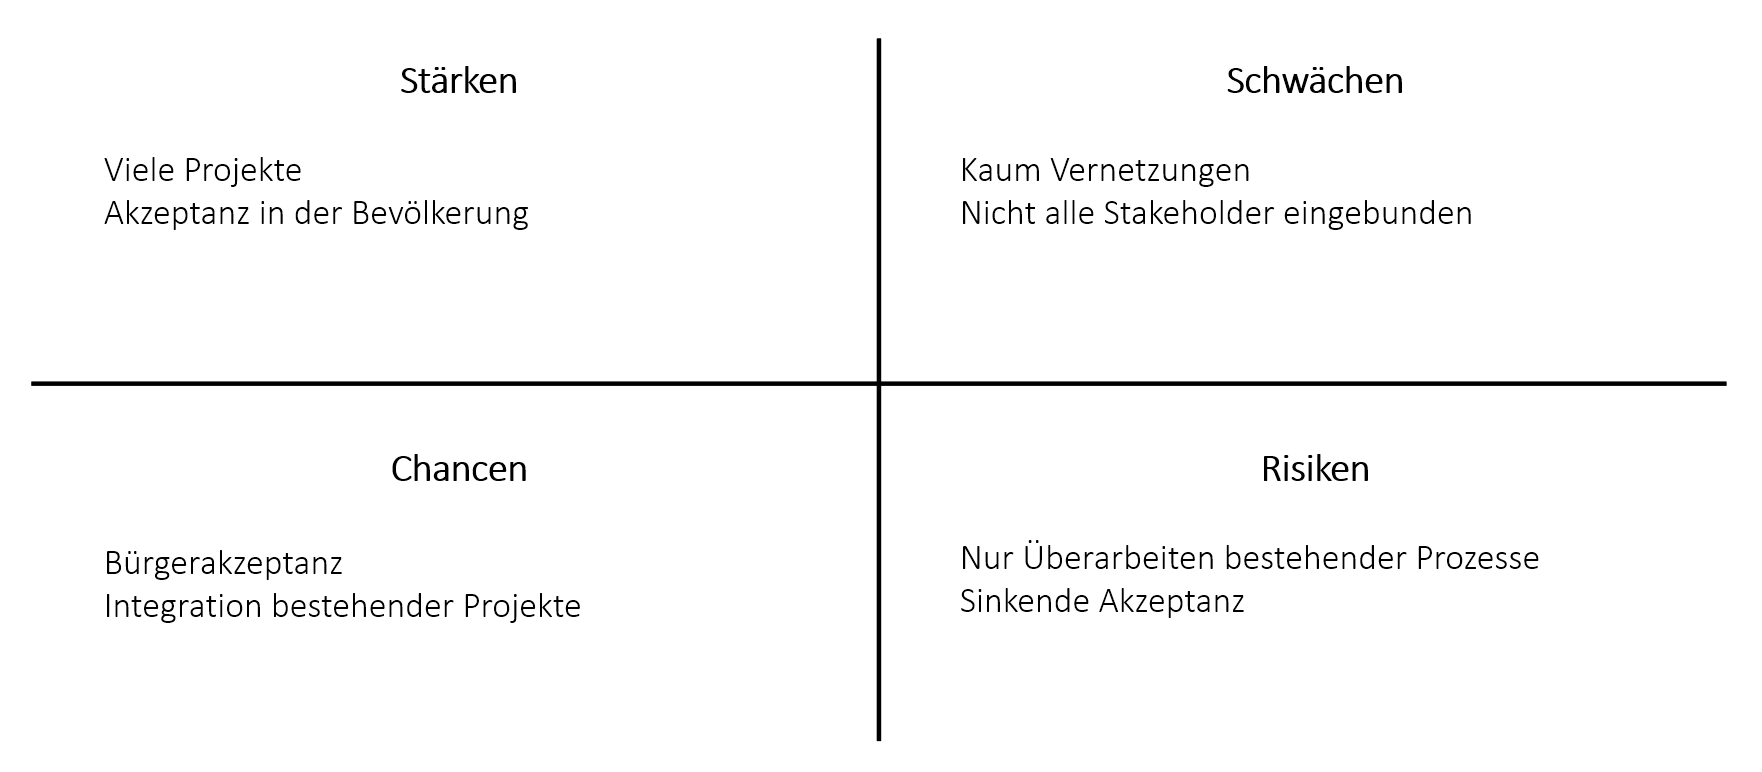
\includegraphics[width=\textwidth]{graphics/5-swot-matrix}
	\caption[SWOT-Matrix zur Entwicklung Hamburgs auf dem Weg zur Smart City]{SWOT-Matrix zur Entwicklung Hamburgs auf dem Weg zur Smart City}
	\label{fig:5_swot_matrix}
\end{figure}

\subsection{Stärken}

Die größte Stärke der hamburger Entwicklungen ist die \textbf{hohe Anzahl der Projekte}. In diesem Bereich sind keine Städte in Deutschland ähnlich fortschrittlich. Dadurch sind Smart-City-Projekte im Alltag der Bürger allgegenwärtig und werden mehr zur Normalität, als wenn nur vereinzelt Projekte durchgeführt werden. Das, und auch sehr erfolgreiche Projekte wie das Transparenzportal, haben zur Folge, dass eine \textbf{hohe Akzeptanz }gegenüber Smart-City-Projekten vorherrscht. Bürger nehmen neu entstehende Projekte so schneller auf und integrieren sie eher in ihren Alltag.

\subsection{Schwächen}

Die hohe Anzahl an Projekten wird in Hamburg jedoch noch nicht optimal ausgenutzt. Viele Projekte integrieren keine anderen Projekte der hamburger Smart-City-Initiative. Dadurch werden \textbf{Synergien nicht genutzt}, die die Effektivität der Projekte weiter steigern könnten. Zusätzlich werden teilweise \textbf{nicht alle Stakeholder mit eingebunden}, die für den Erfolg des Projektes nützlich sein könnten. Eine weitere Schwäche ist der Fokus der Projekte. Manche Projekte fokussieren sich nur auf kurzfristige Problemlösungen ohne die Ursache der Probleme zu ermitteln und zu bekämpfen.

\subsection{Chancen}

Mit Blick auf zukünftige Projekte bietet vor allem die \textbf{hohe Akzeptanz }in der Bevölkerung Chancen in Hamburg. Neue Projekte können mit wenig Aufwand eingeführt werden und können von Bürgern potenziell stärker genutzt werden als in Städten, in denen die Akzeptanz niedriger ist. Zusätzlich bieten aktuelle Schwächen viel Potenzial für Verbesserungen. Die aktuell noch oft siloartig durchgeführten \textbf{Projekte können miteinander verknüpft werden}, um Synergien zu erzeugen und das volle Potenzial der hamburger Smart-City-Projekte auszuschöpfen.

\subsection{Risiken}

Die aktuellen Schwächen des hamburger Smart-City-Konzeptes sollten verbessert werden, sonst können Initiativen des hamburger Senats ihr Potenzial nicht entfalten. Werden die \textbf{Projekte weiterhin siloartig }durchgeführt, kann das für Bürger unübersichtlich wirken und sie eher von neuen Projekten abschrecken. Wird diese Schwäche nicht behoben, kann das die \textbf{Akzeptanz gegenüber den bestehenden und neuen Projekten senken} und die positive Entwicklung entschleunigen.

% - Hauptsächlich aus SWOT-Analyse der Präsentation herausziehen
% - Beispiele einbinden

%Mobility
%- viele Projekte
%- manche greifen ineinander, manche nicht
%  - Hafen nicht, Auto Zug etc gut
%  - Ziel ist der Weltkongress für International Transfer Systems 2021
%- ICTS Weltkongress ist maßgeblich für Mobility-Entwicklungen in Hamburg
%- Beispiel Park'n'joy: Hamburg wird für innovative Projekttests ausgewählt
%  - Weil Akzeptanz in Bevölkerung hoch ist
%- Mobility-Projekte lösen eher langfristige Probleme
%- 